In Exercises \ref{polytransfirst} - \ref{polytranslast}, given the pair of functions $f$ and $F$, sketch the graph of $y=F(x)$ by starting with the graph of $y = f(x)$ and using Theorem \ref{linearmononialgraphs}.  Track at least three points of your choice through the transformations. State the domain and range of $g$.

\begin{multicols}{2}
\begin{enumerate}


\item $f(x) = x^3$,  $F(x) = (x + 2)^{3} + 1$ \label{polytransfirst}
\item $f(x) = x^4$, $F(x) = (x + 2)^{4} + 1$

\setcounter{HW}{\value{enumi}}
\end{enumerate}
\end{multicols}

\begin{multicols}{2}
\begin{enumerate}
\setcounter{enumi}{\value{HW}}

\item $f(x) = x^4$, $F(x) = 2 - 3(x - 1)^{4}$
\item $f(x) = x^5$, $F(x) = -x^{5} - 3$

\setcounter{HW}{\value{enumi}}
\end{enumerate}
\end{multicols}

\begin{multicols}{2}
\begin{enumerate}
\setcounter{enumi}{\value{HW}}

\item $f(x) = x^5$, $F(x) = (x+1)^5+10$
\item $f(x) = x^6$, $F(x) = 8-x^6$ \label{polytranslast}

\setcounter{HW}{\value{enumi}}
\end{enumerate}
\end{multicols}


In Exercises \ref{findformulaforcubicgraphfirst} - \ref{findformulacubicgraphlast}, find a formula for each function below in the form $F(x) = a(x-h)^3+k$.

\begin{multicols}{2}

\begin{enumerate}
\setcounter{enumi}{\value{HW}}

\item $~$ \label{findformulaforcubicgraphfirst}

\begin{mfpic}[15]{-5}{5}{-5}{5}
\axes
\tlabel[cc](5,-0.5){\scriptsize $x$}
\tlabel[cc](0.5,5){\scriptsize $y$}
\tlabel[cc](-1.25, -3){\scriptsize $(0,-3)$}
\tlabel[cc](1.25,-2.75){\scriptsize $(1,-2)$}
\xmarks{-4,-3,-2,-1,1,2,3,4}
\ymarks{-4,-3,-2, -1, 1,2,3,4}
\tlpointsep{4pt}
\scriptsize
\axislabels {x}{ {$-4 \hspace{7pt}$} -4, {$-3 \hspace{7pt}$} -3, {$-2 \hspace{7pt}$} -2, {$-1 \hspace{7pt}$} -1, {$1$} 1, {$2$} 2, {$3$} 3, {$4$} 4}
\axislabels {y}{{$-1$} -1,{$1$} 1, {$2$} 2, {$3$} 3, {$4$} 4, {$-2$} -2}
\penwd{1.25pt}
\arrow \reverse \arrow \function{-0.4,2.9,0.1}{(x-1)**3-2}
\point[4pt]{(1,-2), (0,-3)}
\tcaption{ \scriptsize$y = F(x)$}
\normalsize
\end{mfpic} 



\item $~$ \label{findformulacubicgraphlast}

\begin{mfpic}[15]{-5}{5}{-5}{5}
\axes
\tlabel[cc](5,-0.5){\scriptsize $x$}
\tlabel[cc](0.5,5){\scriptsize $y$}
\tlabel[cc](1,-1){\scriptsize $(0,-1)$}
\tlabel[cc](-2.25,2.25){\scriptsize $(-2,3)$}
\xmarks{-4,-3,-2,-1,1,2,3,4}
\ymarks{-4,-3,-2, -1, 1,2,3,4}
\tlpointsep{4pt}
\scriptsize
\axislabels {x}{ {$-4 \hspace{7pt}$} -4, {$-3 \hspace{7pt}$} -3, {$-2 \hspace{7pt}$} -2, {$-1 \hspace{7pt}$} -1, {$1$} 1, {$2$} 2, {$3$} 3, {$4$} 4}
\axislabels {y}{{$-1$} -1, {$2$} 2, {$3$} 3, {$4$} 4, {$-2$} -2, {$-3$} -3, {$-4$} -4}
\penwd{1.25pt}
\arrow \reverse \arrow \function{-3.5,0.5,0.1}{3-(0.5*((x+2)**3))}
\point[4pt]{(-2,3), (0,-1)}
\tcaption{ \scriptsize$y = F(x)$}
\normalsize
\end{mfpic} 

\setcounter{HW}{\value{enumi}}

\end{enumerate}

\end{multicols}

In Exercises \ref{findformulaforquartgraphfirst} - \ref{findformulaquartgraphlast}, find a formula for each function below in the form $F(x) = a(x-h)^4+k$.


\begin{multicols}{2}

\begin{enumerate}

\setcounter{enumi}{\value{HW}}

\item $~$ \label{findformulaforquartgraphfirst}

\begin{mfpic}[15]{-5}{5}{-5}{5}
\axes
\tlabel[cc](5,-0.5){\scriptsize $x$}
\tlabel[cc](0.5,5){\scriptsize $y$}
\tlabel[cc](-1.25,-4.5){\scriptsize $(-1,-4)$}
\tlabel[cc](1,-2){\scriptsize $(0,-2)$}
\xmarks{-4,-3,-2,-1,1,2,3,4}
\ymarks{-4,-3,-2, -1, 1,2,3,4}
\tlpointsep{4pt}
\scriptsize
\axislabels {x}{ {$-4 \hspace{7pt}$} -4, {$-3 \hspace{7pt}$} -3, {$-1 \hspace{7pt}$} -1, {$1$} 1, {$2$} 2,{$3$} 3, {$4$} 4}
\axislabels {y}{{$-1$} -1,{$1$} 1, {$2$} 2, {$3$} 3,  {$-2$} -2, {$-3$} -3, {$4$} 4}
\penwd{1.25pt}
\arrow \reverse \arrow \function{-2.41,0.41,0.1}{2*((x+1)**4)-4}
\point[4pt]{(-1,-4), (0,-2)}
\tcaption{ \scriptsize$y = F(x)$}
\normalsize
\end{mfpic} 



\item $~$  \label{findformulaquartgraphlast}

\begin{mfpic}[15]{-5}{5}{-5}{5}
\axes
\tlabel[cc](5,-0.5){\scriptsize $x$}
\tlabel[cc](0.5,5){\scriptsize $y$}
\tlabel[cc](-3,0.5){\scriptsize $(-2,0)$}
\tlabel[cc](2.5,0.5){\scriptsize $(2,0)$}
\tlabel[cc](-2,2.5){\scriptsize $(0,2.5)$}
\xmarks{-4,-3,-2,-1,1,2,3,4}
\ymarks{-4,-3,-2, -1, 1,2,3,4}
\tlpointsep{4pt}
\scriptsize
\axislabels {x}{ {$-4 \hspace{7pt}$} -4, {$-3 \hspace{7pt}$} -3, {$-1 \hspace{7pt}$} -1,  {$1$} 1, {$3$} 3, {$4$} 4}
\axislabels {y}{{$-1$} -1,{$-2$} -2,{$-3$} -3,{$-4$} -4,{$1$} 1, {$2$} 2, {$3$} 3,  {$4$} 4}
\penwd{1.25pt}
\arrow \reverse \arrow \function{-2.5,2.5,0.1}{2.5-(0.1565*(x**4))}
\point[4pt]{(-2,0), (2,0), (0, 2.5)}
\tcaption{ \scriptsize$y = F(x)$}
\normalsize
\end{mfpic} 


\setcounter{HW}{\value{enumi}}

\end{enumerate}

\end{multicols}


In Exercises \ref{polyfactsfirst} - \ref{polyfactslast}, find the degree, the leading term, the leading coefficient, the constant term and the end behavior of the given polynomial function.

\begin{multicols}{2}
\begin{enumerate}
\setcounter{enumi}{\value{HW}}
\item  $f(x) = 4-x-3x^2$ \label{polyfactsfirst}
\item  $g(x) = 3x^5 - 2x^2 + x + 1$

\setcounter{HW}{\value{enumi}}
\end{enumerate}
\end{multicols}

\begin{multicols}{2}
\begin{enumerate}
\setcounter{enumi}{\value{HW}}

\item $q(r) = 1 - 16r^{4}$
\item $Z(b) = 42b - b^{3}$

\setcounter{HW}{\value{enumi}}
\end{enumerate}
\end{multicols}

\begin{multicols}{2}
\begin{enumerate}
\setcounter{enumi}{\value{HW}}

\item $f(x) = \sqrt{3}x^{17} + 22.5x^{10} - \pi x^{7} + \frac{1}{3}$
\item $s(t) = -4.9t^{2} + v_{\mbox{\tiny $0$}}t + s_{\mbox{\tiny $0$}}$

\setcounter{HW}{\value{enumi}}
\end{enumerate}
\end{multicols}

\begin{multicols}{2}
\begin{enumerate}
\setcounter{enumi}{\value{HW}}

\item $P(x) = (x - 1)(x - 2)(x - 3)(x - 4)$
\item $p(t) = -t^2(3 - 5t)(t^{2} + t + 4)$

\setcounter{HW}{\value{enumi}}
\end{enumerate}
\end{multicols}

\begin{multicols}{2}
\begin{enumerate}
\setcounter{enumi}{\value{HW}}

\item $f(x) = -2x^3(x+1)(x+2)^2$
\item $G(t) = 4(t-2)^2\left(t+\frac{1}{2}\right)$ \label{polyfactslast}

\setcounter{HW}{\value{enumi}}
\end{enumerate}
\end{multicols}

\phantomsection
\label{polygraphexercise}

In Exercises \ref{zeromultgraphfirst} - \ref{zeromultgraphlast}, find the real zeros of the given polynomial and their corresponding multiplicities.  Use this information along with end behavior to provide a rough sketch of the graph of the polynomial function.  Compare your answer with the result from a graphing utility.

\begin{multicols}{2}
\begin{enumerate}
\setcounter{enumi}{\value{HW}}

\item $a(x) = x(x + 2)^{2}$ \label{zeromultgraphfirst}
\item $g(t) = t(t + 2)^{3}$

\setcounter{HW}{\value{enumi}}
\end{enumerate}
\end{multicols}


\begin{multicols}{2}
\begin{enumerate}
\setcounter{enumi}{\value{HW}}

\item $f(z) = -2(z-2)^2(z+1)$
\item $g(x) = (2x+1)^2(x-3)$

\setcounter{HW}{\value{enumi}}
\end{enumerate}
\end{multicols}


\begin{multicols}{2}
\begin{enumerate}
\setcounter{enumi}{\value{HW}}

\item $F(t) = t^{3}(t+ 2)^{2}$
\item $P(z) = (z- 1)(z - 2)(z - 3)(z - 4)$

\setcounter{HW}{\value{enumi}}
\end{enumerate}
\end{multicols}


\begin{multicols}{2}
\begin{enumerate}
\setcounter{enumi}{\value{HW}}

\item $Q(x) = (x + 5)^{2}(x - 3)^{4}$
\item $h(t) = t^2(t-2)^2(t+2)^2$

\setcounter{HW}{\value{enumi}}
\end{enumerate}
\end{multicols}


\begin{multicols}{2}
\begin{enumerate}
\setcounter{enumi}{\value{HW}}

\item $H(z) = (3-z)(z^2+1)$
\item $Z(x) = x(42 - x^{2})$ \label{zeromultgraphlast}

\setcounter{HW}{\value{enumi}}
\end{enumerate}
\end{multicols}

In Exercises \ref{evenoddornotpolyfirst} - \ref{evenoddornotpolylast}, determine analytically if the following functions are even, odd or neither.  Confirm your answer using a graphing utility.


\begin{multicols}{3}
\begin{enumerate}
\setcounter{enumi}{\value{HW}}

\item $f(x) = 7x$ \label{evenoddornotpolyfirst}
\item $g(t) = 7t + 2$
\item $p(z) = 7$

\setcounter{HW}{\value{enumi}}
\end{enumerate}
\end{multicols}

\begin{multicols}{3}
\begin{enumerate}
\setcounter{enumi}{\value{HW}}

\item $F(s) = 3s^2 - 4$
\item $h(t) = 4-t^2$
\item $g(x) = x^2-x-6$

\setcounter{HW}{\value{enumi}}
\end{enumerate}
\end{multicols}


\begin{multicols}{3}
\begin{enumerate}
\setcounter{enumi}{\value{HW}}

\item $f(x) = 2x^3 - x$
\item $p(z) = -z^5 + 2z^3 - z$
\item $G(t) = t^{6} - t^{4} + t^{2} + 9$

\setcounter{HW}{\value{enumi}}
\end{enumerate}
\end{multicols}

\begin{multicols}{3}
\begin{enumerate}
\setcounter{enumi}{\value{HW}}

\item $G(s) = s(s^2 - 1)$
\item $f(x) = (x^2+1)(x-1)$
\item $H(t) = (t^2-1)(t^4+t^2+3)$

\setcounter{HW}{\value{enumi}}
\end{enumerate}
\end{multicols}

\begin{multicols}{3}
\begin{enumerate}
\setcounter{enumi}{\value{HW}}

\item $g(t) = t(t-2)(t+2)$
\item $P(z) = (2z^{5} - 3z)(5z^3+z)$ 
\item $f(x) =0$  \label{evenoddornotpolylast}

\setcounter{HW}{\value{enumi}}
\end{enumerate}
\end{multicols}


\begin{enumerate}
\setcounter{enumi}{\value{HW}}

\item  \label{evenoddpolynomialexercise} Suppose $p(x)$ is a polynomial function written in the form of  Definition \ref{polynomialfunction}.  

\begin{enumerate}

\item  If the nonzero terms of $p(x)$ consist of even powers of $x$ (or a constant), explain why $p$ is even.

\item   If the nonzero terms of $p(x)$ consist of odd powers of $x$, explain why $p$ is odd.

\item  If $p(x)$ the nonzero terms of $p(x)$  contain at least one odd power of $x$ and one even power of $x$ (or a constant term), then $p$ is neither even nor odd.

\end{enumerate}

\newpage

\item  Use the results of Exercise \ref{evenoddpolynomialexercise} to determine whether the following functions are even, odd, or neither.

\begin{multicols}{4}
\begin{enumerate}

\item  $p(x) = 3x^4 + x^2 - 1$

\item  $F(s) = s^3 - 14s$

\item  $f(t) = 2t^5 - t^2 + 1$

\item  $g(x) =x^3(x^2+1)$

\end{enumerate}

\end{multicols}

\item  Show  $f(x) = |x|$ is an even function.


\item  Rework Example \ref{boxnotopex} assuming the box is to be made from an 8.5 inch by 11 inch sheet of paper. Using scissors and tape, construct the box.  Are you surprised?\footnote{Consider decorating the box and presenting it to your instructor. If done well enough, maybe your instructor will issue you some bonus points.  Or maybe not.}

\item For each function $f(x)$ listed below, compute the average rate of change over the indicated interval.\footnote{See Definition \ref{arc} in Section \ref{AverageRateofChange} for a review of this concept, as needed.}  What trends do you observe?  How do your answers manifest themselves graphically?

\[ \begin{array}{|r||c|c|c|c|c|c|}  \hline

 f(x) &  [-0.1, 0] & [0, 0.1] &[0.9, 1] & [1, 1.1] & [1.9, 2] & [2, 2.1]  \\ \hline
 1 &&&&&& \\  \hline
 x  &&&&&& \\  \hline
 x^2 &&&&&&  \\  \hline
 x^3 &&&&&& \\  \hline
 x^4 &&&&&& \\ \hline
 x^5 &&&&&& \\ \hline

\end{array} \]


\item \label{monomialarcexercise}For each function $f(x)$ listed below, compute the average rate of change over the indicated interval.\footnote{See Definition \ref{arc} in Section \ref{AverageRateofChange} for a review of this concept, as needed.}  What trends do you observe?  How do your answers manifest themselves graphically?

\[ \begin{array}{|r||c|c|c|c|}  \hline

 f(x) &  [0.9, 1.1] & [0.99, 1.01] &[0.999, 1.001] & [0.9999, 1.0001]  \\ \hline
 1 &&&&   \\  \hline
 x &&&&    \\  \hline
 x^2 &&&&   \\  \hline
 x^3 &&&&   \\  \hline
 x^4 &&&&  \\ \hline
 x^5 &&&&  \\ \hline

\end{array} \]




\setcounter{HW}{\value{enumi}}
\end{enumerate}

\phantomsection
\label{LCDmaxprofit} 

In Exercises \ref{lcdmaxprofitexerfirst} - \ref{lcdmaxprofitexerlast}, suppose the revenue $R$, in \textit{thousands} of dollars, from producing and selling $x$ \textit{hundred} LCD TVs is given by $R(x) = -5x^3+35x^2+155x$ for $0 \leq x \leq 10.07$.

\begin{enumerate}
\setcounter{enumi}{\value{HW}}

\item  Use a graphing utility to graph $y = R(x)$ and determine the number of TVs which should be sold to maximize revenue.  What is the maximum revenue? \label{lcdmaxprofitexerfirst}

\item Assume the cost, in \textit{thousands} of dollars, to produce $x$ \textit{hundred} LCD TVs is given by the function $C(x) = 200x + 25$ for $x \geq 0$. Find and simplify an expression for the profit function $P(x)$.  

(Remember: Profit = Revenue - Cost.)

\item  Use a graphing utility to graph $y = P(x)$ and determine the number of TVs which should be sold to maximize profit.  What is the maximum  profit? \label{lcdmaxprofitexerlast}

\item \label{newportaboycost} While developing their newest game, Sasquatch Attack!, the makers of the PortaBoy (from Example \ref{PortaBoyCost}) revised their cost function and now use $C(x) = .03x^{3} - 4.5x^{2} + 225x + 250$, for $x \geq 0$. As before, $C(x)$ is the cost to make $x$ PortaBoy Game Systems.  Market research indicates that the demand function $p(x) = -1.5x + 250$ remains unchanged.  Use a graphing utility to find the production level $x$ that maximizes the \textit{profit} made by producing and selling $x$ PortaBoy game systems.

\setcounter{HW}{\value{enumi}}
\end{enumerate}

\begin{enumerate}
\setcounter{enumi}{\value{HW}}

\item According to US Postal regulations, a rectangular shipping box must satisfy the following inequality: ``Length + Girth $\leq$ 130 inches'' for Parcel Post and ``Length + Girth $\leq$ 108 inches'' for other services. 

\smallskip

Let's assume we have a closed rectangular box with a square face of side length $x$ as drawn below.  The length is the longest side and is clearly labeled.  The girth is the distance around the box in the other two dimensions so in our case it is the sum of the four sides of the square, $4x$.  

\begin{enumerate}

\item \label{girthbox1} Assuming that we'll be mailing a box via Parcel Post where Length + Girth $=$ 130 inches, express the length of the box in terms of $x$ and then express the volume $V$ of the box in terms of $x$.

\item \label{girthbox2} Find the dimensions of the box of maximum volume that can be shipped via Parcel Post.

\item Repeat parts \ref{girthbox1} and \ref{girthbox2} if the box is shipped using ``other services''.

\end{enumerate}

\begin{center}

\begin{mfpic}[8]{-6}{12}{-1}{17}
\polyline{(0,0),(-4,3)}
\polyline{(-4,3), (-4,8)}
\polyline{(-4,8),(0,5)}
\polyline{(0,5),(0,0)}
\polyline{(0,0),(12,9)}
\polyline{(0,5),(12,14)}
\polyline{(-4,8),(8,17)}
\polyline{(8,17),(12,14)}
\polyline{(12,14),(12,9)}
\arrow \reverse \arrow \polyline{(0,-0.5),(12,8.5)}
\tlabel[cc](8,4){\tiny length}
\arrow \reverse \arrow \polyline{(-4, 2.5), (-0.5,-0.125)}
\tlabel[cc](-3,0.5){\tiny $x$}
\arrow \reverse \arrow \polyline{(-4.5, 3), (-4.5,8)}
\tlabel[cc](-5,5){\tiny $x$}
\end{mfpic}

\end{center}

\setcounter{HW}{\value{enumi}}
\end{enumerate}

\newpage

\begin{enumerate}
\setcounter{enumi}{\value{HW}}


\item \label{sunlighthigherorder} This exercise revisits the data set from Exercise \ref{regsunlight} in Section \ref{QuadraticFunctions}.  In that exercise, you were given a chart of the number of hours of daylight they get on the $21^{\mbox{st}}$ of each month in Fairbanks, Alaska based on the 2009 sunrise and sunset data found on the  \href{http://aa.usno.navy.mil/data/docs/RS_OneYear.php}{\underline{U.S. Naval Observatory}} website.  Here  $x = 1$ represents January 21, 2009, $x = 2$ represents February 21, 2009, and so on.  
\medskip

\small

\noindent \begin{tabular}{|l|r|r|r|r|r|r|r|r|r|r|r|r|} \hline
Month  & & & & & & & & & & & & \\
Number & 1 & 2 & 3 & 4 & 5 & 6 & 7 & 8 & 9 & 10 & 11 & 12\\ 
\hline 
Hours of  & & & & & & & & & & & & \\
Daylight & 5.8 & 9.3 & 12.4 & 15.9 & 19.4 & 21.8 & 19.4 & 15.6 & 12.4 & 9.1 & 5.6 & 3.3 \\ \hline
\end{tabular}

\normalsize

\medskip

\noindent 

\begin{itemize}

\item Find cubic (third degree) and quartic (fourth degree) polynomials which model this data and comment on the goodness of fit for each.  What can we say about using either model to make predictions about the year 2020?  (Hint: Think about the end behavior of polynomials.)  

\item Use the models to see how many hours of daylight they got on your birthday and then check the website to see how accurate the models are.  

\item Sasquatch are largely nocturnal, so what days of the year according to your models  allow for at least 14 hours of darkness for field research on the elusive creatures? 

\end{itemize}

\item \label{circuitexercisepoly} An electric circuit is built with a variable resistor installed.  For each of the following resistance values (measured in kilo-ohms, $k \Omega$),  the corresponding power to the load (measured in milliwatts, $mW$) is given in the table below. \footnote{The authors wish to thank Don Anthan and Ken White of Lakeland Community College for devising this problem and generating the accompanying data set.}

\noindent \begin{tabular}{|l|r|r|r|r|r|r|} \hline
Resistance: ($k \Omega$) & 1.012 & 2.199 & 3.275 & 4.676 & 6.805 & 9.975 \\ \hline
Power: ($mW$) & 1.063 & 1.496 & 1.610 & 1.613 & 1.505 & 1.314 \\ \hline
\end{tabular}

\begin{enumerate}

\item Make a scatter diagram of the data using the Resistance as the independent variable and Power as the dependent variable.

\item Use your calculator to find quadratic (2nd degree), cubic (3rd degree) and quartic (4th degree) regression models for the data and judge the reasonableness of each.

\item For each of the models found above, find the predicted maximum power that can be delivered to the load.  What is the corresponding resistance value?

\item Discuss with your classmates the limitations of these models - in particular, discuss the end behavior of each.

\end{enumerate}

\newpage

\item Below is a graph of  a polynomial function $y = p(x)$ as generated by a graphing utility.   Answer the following questions about $p$ based on the graph provided.


\centerline{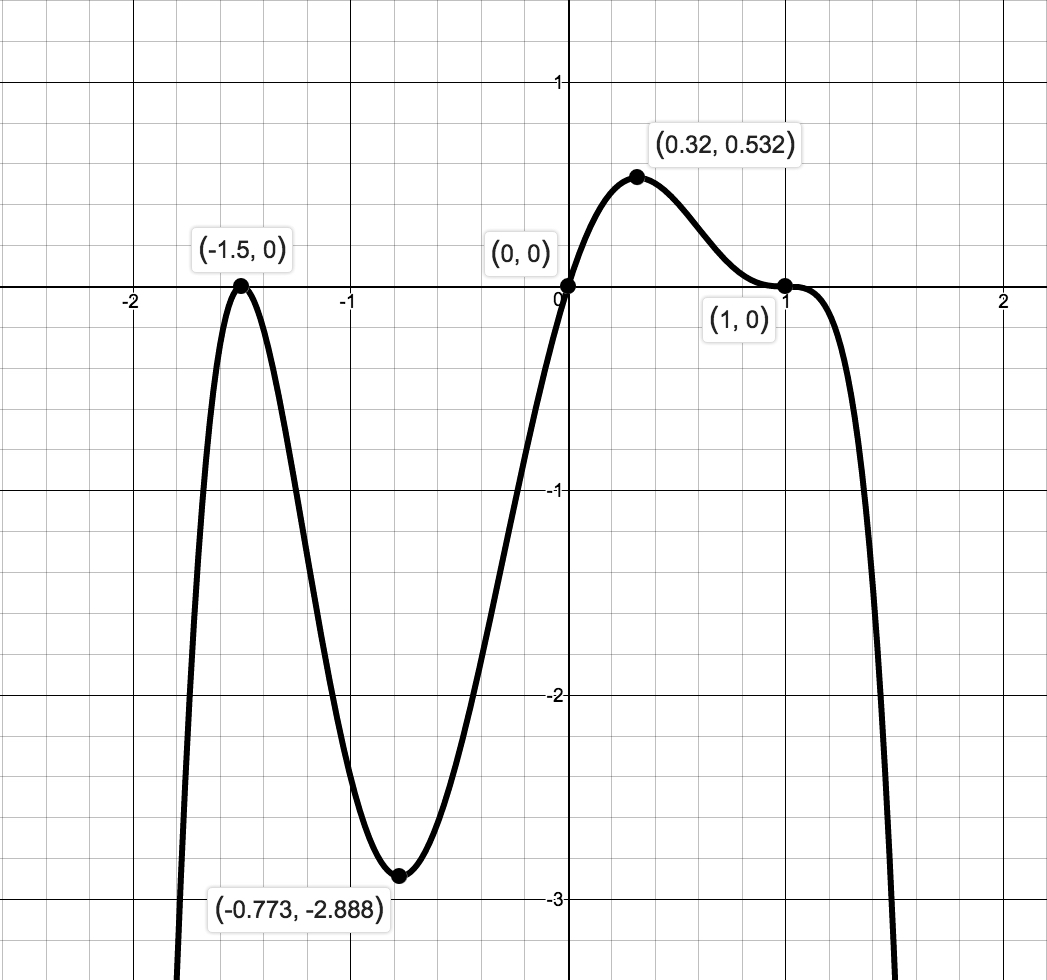
\includegraphics[width=3in]{./GraphsofPolynomialsGraphics/GraphsofPolyExercise.jpg}}

\begin{enumerate}

\item  Describe the end behavior of $y = p(x)$.

\item  List the real zeros of $p$ along with their respective multiplicities.  

\item  List the local minimums and local maximums of the graph of $y = p(x)$.

\item  What can be said about the degree of and leading coefficient $p(x)$?

\item  It turns out that $p(x)$ is a seventh degree polynomial.\footnote{to be exact, $p(x) = -0.1\left(x+1.5\right)^2\left(3x\right)\left(x-1\right)^3\left(x+5\right)$.}  How can this be?

\end{enumerate}

\item  \label{comparegraphfromtheoryexample}  (This Exercise is a follow up to Example \ref{graphfromtheory}.)  Use a graphing utility to  compare and contrast the graphs of $f(x) = (2x-1)(x+1)^2(1-x)(x^2+1)$ and $g(x) = (2x-1)(x+1)^2(1-x)$.

\item Use the graph of $y= p(x) = (2x-1)(x+1)(1-x^4)$ on page \pageref{localmaxminexample} to estimate the largest open interval containing $x = -0.235$ which satisfies the the criteria for `local minimum'  in Definition \ref{localmaxmindefn}.

\item  In light of Definition \ref{localmaxmindefn}, explain why \textit{every} point on the graph of a constant function is both a local maximum and a local minimum.

\item This exercise involves the greatest integer function, $f(x) = \lfloor x \rfloor$,  introduced in Example \ref{greatestintegerdefn}.  Explain why the points $(k,k)$ for integers $k$ are local maximums but not local minimums.

\item  Use Theorems  \ref{EBPolynomials}  and \ref{polynomialbehaviornearzeros} prove Theorem \ref{roleofmultiplicity}.


\newpage

\item Here are a few other questions for you to discuss with your classmates.  

\begin{enumerate}

\item How many and how few  local extrema could a polynomial of degree $n$ have?  
\item Could a polynomial have two local maxima but no local minima?  
\item If a polynomial has two local maxima and two local minima, can it be of odd degree?  Can it be of even degree?
\item Can a polynomial have local extrema without having any real zeros?
\item Why must every polynomial of odd degree have at least one real zero?
\item Can a polynomial have two distinct real zeros and no local extrema?
\item Can an $x$-intercept yield a local extrema?  Can it yield an absolute extrema?
\item If the $y$-intercept yields an absolute minimum, what can we say about the degree of the polynomial and the sign of the leading coefficient?   

\end{enumerate}

\item \label{LagrangePolyExercise} (This is a follow-up to Exercises \ref{LagrangeLinearExercise} in Section \ref{ConstantandLinearFunctions} and \ref{LagrangeQuadExercise} in Section \ref{QuadraticFunctions}.) The  \href{https://en.wikipedia.org/wiki/Lagrange_polynomial}{\underline{Lagrange Interpolate}} function $L$  for four  points:  $(x_{0}, y_{0})$, $(x_{1}, y_{1})$,  $(x_{2}, y_{2})$,   $(x_{3}, y_{3})$ where $x_{0}$,  $x_{1}$, $x_{2}$, and $x_{3}$ are four distinct real numbers is given by the formula: 

 \[ \begin{array}{rcl}
 
 L(x) & = &  y_{0}  \dfrac{(x - x_{1}) (x - x_{2}) (x-x_{3})}{(x_{0} - x_{1})(x_{0} - x_{2})(x_{0} - x_{3})}+ y_{1}  \dfrac{(x - x_{0}) (x - x_{2}) (x-x_{3})}{(x_{1} - x_{0})(x_{1} - x_{2})(x_{1} - x_{3})} \\ [15pt]
         &&  +y_{2}  \dfrac{(x - x_{0}) (x - x_{1}) (x-x_{3})}{(x_{2} - x_{0})(x_{2} - x_{1})(x_{2} - x_{3})}+ y_{3}  \dfrac{(x - x_{0}) (x - x_{1}) (x-x_{2})}{(x_{3} - x_{0})(x_{3} - x_{1})(x_{3} - x_{2})} \\ \end{array}\]

\begin{enumerate}

\item Choose four points with different $x$-values and construct the Lagrange Interpolate for those points.  Verify each of the points lies on the polynomial.  

\item  Verify that, in general, $L(x_{0}) = y_{0}$,  $L(x_{1}) = y_{1}$, $L(x_{2}) = y_{2}$, and  $L(x_{3}) = y_{3}$.

\item  Find $L(x)$ for the points $(-1,1)$, $(0,0)$,  $(1,1)$ and $(2,4)$.  What happens?

\item  Find $L(x)$ for the points $(-1,0)$, $(0,1)$,  $(1,2)$ and $(2,3)$.  What happens?

\item  Generalize the formula for $L(x)$ to five points.  What's the pattern?

\end{enumerate}

\setcounter{HW}{\value{enumi}}
\end{enumerate}
\newpage

\subsection{Answers}

\begin{multicols}{2}
\begin{enumerate}


\item $F(x) = (x + 2)^{3} + 1$ \\ 
domain: $(-\infty, \infty)$ \\ 
range: $(-\infty, \infty)$ \\

\begin{mfpic}[20][8]{-5}{1}{-11}{13}
\axes
\tlabel[cc](1,-0.75){\scriptsize $x$}
\tlabel[cc](0.5,13){\scriptsize $y$}
\point[4pt]{(-4,-7),(-3,0),(-2,1),(-1,2),(0,9)}
\xmarks{-4,-3,-2,-1}
\ymarks{-10 step 1 until 12}
\tiny
\tlpointsep{4pt}
\axislabels {x}{{$-4 \hspace{6pt}$} -4, {$-3 \hspace{6pt}$} -3, {$-2 \hspace{6pt}$} -2, {$-1 \hspace{6pt}$} -1}
\axislabels {y}{{$-10$} -10, {$-9$} -9, {$-8$} -8, {$-7$} -7, {$-6$} -6, {$-5$} -5, {$-4$} -4, {$-3$} -3, {$-2$} -2, {$-1$} -1, {$1$} 1, {$2$} 2, {$3$} 3, {$4$} 4, {$5$} 5, {$6$} 6, {$7$} 7, {$8$} 8, {$9$} 9, {$10$} 10, {$11$} 11, {$12$} 12}
\normalsize
\penwd{1.25pt}
\arrow \reverse \arrow \function{-4.25,0.25,0.1}{((x + 2)**3) + 1}
\end{mfpic}

\vfill

\columnbreak

\item $F(x) = (x + 2)^{4} + 1$\\
domain: $(-\infty, \infty)$\\
range: $[1, \infty)$\\

\begin{mfpic}[20][8]{-5}{1}{-1}{22}
\axes
\tlabel[cc](1,-0.75){\scriptsize $x$}
\tlabel[cc](0.5,22){\scriptsize $y$}
\point[4pt]{(-4,17),(-3,2),(-2,1),(-1,2),(0,17)}
\xmarks{-4,-3,-2,-1}
\ymarks{1 step 1 until 21}
\tiny
\tlpointsep{4pt}
\axislabels {x}{{$-4 \hspace{6pt}$} -4, {$-3 \hspace{6pt}$} -3, {$-2 \hspace{6pt}$} -2, {$-1 \hspace{6pt}$} -1}
\axislabels {y}{{$1$} 1, {$2$} 2, {$3$} 3, {$4$} 4, {$5$} 5, {$6$} 6, {$7$} 7, {$8$} 8, {$9$} 9, {$10$} 10, {$11$} 11, {$12$} 12, {$13$} 13, {$14$} 14, {$15$} 15, {$16$} 16, {$17$} 17, {$18$} 18, {$19$} 19, {$20$} 20, {$21$} 21}
\normalsize
\penwd{1.25pt}
\arrow \reverse \arrow \function{-4.12,0.12,0.1}{((x + 2)**4) + 1}
\end{mfpic}

\setcounter{HW}{\value{enumi}}
\end{enumerate}
\end{multicols}

\begin{multicols}{2}
\begin{enumerate}
\setcounter{enumi}{\value{HW}}


\item $F(x) = 2 - 3(x - 1)^{4}$\\
domain: $(-\infty, \infty)$\\
range: $(-\infty, 2]$\\

\begin{mfpic}[20][8]{-1}{3}{-14}{3}
\axes
\tlabel[cc](3,-0.75){\scriptsize $x$}
\tlabel[cc](0.5,3){\scriptsize $y$}
\point[4pt]{(1,2),(0,-1),(2,-1)}
\xmarks{1,2}
\ymarks{-13 step 1 until 2}
\tiny
\tlpointsep{4pt}
\axislabels {x}{{$1$} 1, {$2$} 2}
\axislabels {y}{{$-13$} -13, {$-12$} -12, {$-11$} -11, {$-10$} -10, {$-9$} -9, {$-8$} -8, {$-7$} -7, {$-6$} -6, {$-5$} -5, {$-4$} -4, {$-3$} -3, {$-2$} -2, {$-1$} -1, {$1$} 1, {$2$} 2}
\normalsize
\penwd{1.25pt}
\arrow \reverse \arrow \function{-0.5,2.5,0.1}{2 - 3*((x - 1)**4)}
\end{mfpic}


\vfill

\columnbreak

\item $F(x) = -x^{5} - 3$\\
domain: $(-\infty, \infty)$\\
range: $(-\infty, \infty)$\\

\begin{mfpic}[20][8]{-2}{2}{-11}{11}
\axes
\tlabel[cc](2,-0.75){\scriptsize $x$}
\tlabel[cc](0.5,11){\scriptsize $y$}
\point[4pt]{(-1,-2),(0,-3),(1,-4)}
\xmarks{-1,1}
\ymarks{-10 step 1 until 10}
\tiny
\tlpointsep{4pt}
\axislabels {x}{{$-1 \hspace{6pt}$} -1, {$1$} 1}
\axislabels {y}{{$-10$} -10, {$-9$} -9, {$-8$} -8, {$-7$} -7, {$-6$} -6, {$-5$} -5, {$-4$} -4, {$-3$} -3, {$-2$} -2, {$-1$} -1, {$1$} 1, {$2$} 2, {$3$} 3, {$4$} 4, {$5$} 5, {$6$} 6, {$7$} 7, {$8$} 8, {$9$} 9, {$10$} 10}
\normalsize
\penwd{1.25pt}
\arrow \reverse \arrow \function{-1.68,1.5,0.1}{-(x**5) - 3}
\end{mfpic}


\setcounter{HW}{\value{enumi}}
\end{enumerate}
\end{multicols}


\pagebreak

\begin{multicols}{2}
\begin{enumerate}

\setcounter{enumi}{\value{HW}}
\item $F(x) = (x+1)^5+10$\\
domain: $(-\infty, \infty)$\\
range: $(-\infty, \infty)$\\

\begin{mfpic}[20][8]{-5}{1}{-1}{22}
\axes
\tlabel[cc](1,-0.75){\scriptsize $x$}
\tlabel[cc](0.5,22){\scriptsize $y$}
\point[4pt]{(0,11), (-1,10), (-2,9)}
\xmarks{-4,-3,-2,-1}
\ymarks{1 step 1 until 21}
\tiny
\tlpointsep{4pt}
\axislabels {x}{{$-4 \hspace{6pt}$} -4, {$-3 \hspace{6pt}$} -3, {$-2 \hspace{6pt}$} -2, {$-1 \hspace{6pt}$} -1}
\axislabels {y}{{$1$} 1, {$2$} 2, {$3$} 3, {$4$} 4, {$5$} 5, {$6$} 6, {$7$} 7, {$8$} 8, {$9$} 9, {$10$} 10, {$11$} 11, {$12$} 12, {$13$} 13, {$14$} 14, {$15$} 15, {$16$} 16, {$17$} 17, {$18$} 18, {$19$} 19, {$20$} 20, {$21$} 21}
\normalsize
\penwd{1.25pt}
\arrow \reverse \arrow \function{-2.64,0.58,0.1}{((x + 1)**5) + 10}
\end{mfpic}


\vfill

\columnbreak

\item $F(x) = 8-x^{6}$\\
domain: $(-\infty, \infty)$\\
range: $(-\infty, 8]$\\

\begin{mfpic}[20][8]{-2}{2}{-11}{11}
\axes
\tlabel[cc](2,-0.75){\scriptsize $x$}
\tlabel[cc](0.5,11){\scriptsize $y$}
\point[4pt]{(-1,7),(0,8),(1,7)}
\xmarks{-1,1}
\ymarks{-10 step 1 until 10}
\tiny
\tlpointsep{4pt}
\axislabels {x}{{$-1 \hspace{6pt}$} -1, {$1$} 1}
\axislabels {y}{{$-10$} -10, {$-9$} -9, {$-8$} -8, {$-7$} -7, {$-6$} -6, {$-5$} -5, {$-4$} -4, {$-3$} -3, {$-2$} -2, {$-1$} -1, {$1$} 1, {$2$} 2, {$3$} 3, {$4$} 4, {$5$} 5, {$6$} 6, {$7$} 7, {$8$} 8, {$9$} 9, {$10$} 10}
\normalsize
\penwd{1.25pt}
\arrow \reverse \arrow \function{-1.6,1.6,0.1}{8-(x**6)}
\end{mfpic}


\setcounter{HW}{\value{enumi}}
\end{enumerate}
\end{multicols}


\begin{multicols}{2}
\begin{enumerate}
\setcounter{enumi}{\value{HW}}

\item  $F(x) = (x-1)^3-2$ \vphantom{$F(x) = -\frac{1}{2} (x+2)^3+3$}
\item $F(x) = -\frac{1}{2} (x+2)^3+3$

\setcounter{HW}{\value{enumi}}
\end{enumerate}
\end{multicols}

\begin{multicols}{2}
\begin{enumerate}
\setcounter{enumi}{\value{HW}}

\item  $F(x) = 2(x+1)^4-4$ \
\item $F(x) = -0.15625x^4+2.5$

\setcounter{HW}{\value{enumi}}
\end{enumerate}
\end{multicols}


\begin{multicols}{2}
\begin{enumerate}
\setcounter{enumi}{\value{HW}}
\item $f(x) = 4-x-3x^2$ \\
Degree 2 \\
Leading term $-3x^{2}$\\
Leading coefficient $-3$\\
Constant term $4$\\
$\ds{\lim_{x \rightarrow - \infty} f(x)  = -\infty}$ \\
$\ds{\lim_{x \rightarrow  \infty} f(x)  = -\infty}$ \\


\item  $g(x) = 3x^5 - 2x^2 + x + 1$ \\
Degree 5 \\
Leading term $3x^5$\\
Leading coefficient $3$\\
Constant term $1$\\
$\ds{\lim_{x \rightarrow - \infty} g(x)  = -\infty}$ \\
$\ds{\lim_{x \rightarrow \infty} g(x)  = \infty}$ \\



\setcounter{HW}{\value{enumi}}
\end{enumerate}
\end{multicols}

\begin{multicols}{2}
\begin{enumerate}
\setcounter{enumi}{\value{HW}}

\item $q(r) = 1 - 16r^{4}$\\
Degree 4 \\
Leading term $-16r^{4}$\\
Leading coefficient $-16$\\
Constant term $1$\\
$\ds{\lim_{r \rightarrow - \infty} q(r)  = -\infty}$ \\
$\ds{\lim_{r \rightarrow \infty} q(r)  = -\infty}$ \\


\item $Z(b) = 42b - b^{3}$\\
Degree 3 \\
Leading term $-b^{3}$\\
Leading coefficient $-1$\\
Constant term $0$\\
$\ds{\lim_{b \rightarrow - \infty} Z(b)  = \infty}$ \\
$\ds{\lim_{b \rightarrow  \infty} Z(b)  =  - \infty}$ \\

\setcounter{HW}{\value{enumi}}
\end{enumerate}
\end{multicols}

\begin{multicols}{2}
\begin{enumerate}
\setcounter{enumi}{\value{HW}}

\item $f(x) = \sqrt{3}x^{17} + 22.5x^{10} - \pi x^{7} + \frac{1}{3}$\\
Degree 17 \\
Leading term $\sqrt{3}x^{17}$\\
Leading coefficient $\sqrt{3}$\\
Constant term $\frac{1}{3}$\\
$\ds{\lim_{x \rightarrow - \infty} f(x)  = -\infty}$ \\
$\ds{\lim_{x \rightarrow  \infty} f(x)  = \infty}$ \\



\item $s(t) = -4.9t^{2} + v_{\mbox{\tiny $0$}}t + s_{\mbox{\tiny $0$}}$\\
Degree 2 \\
Leading term $-4.9t^{2}$\\
Leading coefficient $-4.9$\\
Constant term $s_{\mbox{\tiny $0$}}$\\
$\ds{\lim_{t \rightarrow - \infty} s(t)  = -\infty}$ \\
$\ds{\lim_{t \rightarrow  \infty} s(t)  = -\infty}$ \\



\setcounter{HW}{\value{enumi}}
\end{enumerate}
\end{multicols}

\begin{multicols}{2}
\begin{enumerate}
\setcounter{enumi}{\value{HW}}


\item $P(x) = (x - 1)(x - 2)(x - 3)(x - 4)$\\
Degree 4 \\
Leading term $x^{4}$\\
Leading coefficient $1$\\
Constant term $24$\\
$\ds{\lim_{x \rightarrow - \infty} P(x)  = \infty}$ \\
$\ds{\lim_{x \rightarrow  \infty} P(x)  = -\infty}$ \\


\item $p(t) = -t^2(3 - 5t)(t^{2} + t + 4)$\\
Degree 5 \\
Leading term $5t^{5}$\\
Leading coefficient $5$\\
Constant term $0$\\
$\ds{\lim_{t \rightarrow - \infty} p(t)  = -\infty}$ \\
$\ds{\lim_{t \rightarrow  \infty} p(t)  = \infty}$ \\

\setcounter{HW}{\value{enumi}}
\end{enumerate}
\end{multicols}



\begin{multicols}{2}
\begin{enumerate}
\setcounter{enumi}{\value{HW}}

\item $f(x) = -2x^3(x+1)(x+2)^2$ \\
Degree 6 \\
Leading term $-2x^{6}$\\
Leading coefficient $-2$\\
Constant term $0$\\
$\ds{\lim_{x \rightarrow - \infty} f(x)  = -\infty}$ \\
$\ds{\lim_{x \rightarrow  \infty} f(x)  = -\infty}$ \\

\item $G(t) = 4(t-2)^2\left(t+\frac{1}{2}\right)$ \\
Degree 3 \\
Leading term $4t^3$\\
Leading coefficient $4$\\
Constant term $8$\\
$\ds{\lim_{t \rightarrow - \infty} G(t)  = -\infty}$ \\
$\ds{\lim_{t \rightarrow  \infty} G(t)  = \infty}$ \\


\setcounter{HW}{\value{enumi}}
\end{enumerate}
\end{multicols}

\begin{multicols}{2}
\begin{enumerate}
\setcounter{enumi}{\value{HW}}

\item $a(x) = x(x + 2)^{2}$\\
$x = 0$ multiplicity 1\\
$x = -2$ multiplicity 2\\

\begin{mfpic}[20][10]{-3}{1}{-3}{5}
\axes
\tlabel[cc](1,-0.5){\scriptsize $x$}
\tlabel[cc](0.25,5){\scriptsize $y$}
\point[4pt]{(-2,0), (0,0)}
\xmarks{-2,-1}
\tiny
\tlpointsep{4pt}
\axislabels {x}{{$-2 \hspace{6pt}$} -2, {$-1 \hspace{6pt}$} -1}
\normalsize
\penwd{1.25pt}
\arrow \reverse \arrow \function{-3,0.65,0.1}{x*((x + 2)**2)}
\end{mfpic}

\vfill

\columnbreak

\item $g(t) = t(t + 2)^{3}$\\
$t = 0$ multiplicity 1\\
$t = -2$ multiplicity 3\\

\begin{mfpic}[20][20]{-3}{1}{-2}{5}
\axes
\tlabel[cc](1,-0.5){\scriptsize $t$}
\tlabel[cc](0.25,5){\scriptsize $y$}
\point[4pt]{(-2,0), (0,0)}
\xmarks{-2,-1}
\tiny
\tlpointsep{4pt}
\axislabels {x}{{$-2 \hspace{6pt}$} -2, {$-1 \hspace{6pt}$} -1}
\normalsize
\penwd{1.25pt}
\arrow \reverse \arrow \function{-3,0.3,0.1}{x*((x + 2)**3)}
\end{mfpic}


\setcounter{HW}{\value{enumi}}
\end{enumerate}
\end{multicols}

\begin{multicols}{2}
\begin{enumerate}
\setcounter{enumi}{\value{HW}}

\item $f(z) = -2(z-2)^2(z+1)$\\
$z=2$ multiplicity 2 \\
$z=-1$ multiplicity 1\\

\begin{mfpic}[20][10]{-3}{3}{-4}{4}
\axes
\tlabel[cc](3,-0.5){\scriptsize $z$}
\tlabel[cc](0.25,4){\scriptsize $y$}
\point[4pt]{(2,0), (-1,0)}
\xmarks{-2,-1,1,2}
\tiny
\tlpointsep{4pt}
\axislabels {x}{{$-2 \hspace{6pt}$} -2, {$-1 \hspace{6pt}$} -1, {$1$} 1, {$2$} 2}
\normalsize
\penwd{1.25pt}
\arrow \reverse \arrow \function{-1.70,3.45,0.1}{(-0.4)*((x-2)**2)*(x+1)}
\end{mfpic}



\item $g(x) = (2x+1)^2(x-3)$\\
$x=-\frac{1}{2}$ multiplicity 2 \\
$x=3$ multiplicity 1\\

\begin{mfpic}[20][10]{-2}{4}{-4}{4}
\axes
\tlabel[cc](4,-0.5){\scriptsize $x$}
\tlabel[cc](0.25,4){\scriptsize $y$}
\point[4pt]{(-0.5,0), (3,0)}
\xmarks{-1,1,2,3}
\tiny
\tlpointsep{4pt}
\axislabels {x}{{$-1 \hspace{6pt}$} -1, {$1$} 1, {$2$} 2, {$3$} 3}
\normalsize
\penwd{1.25pt}
\arrow \reverse \arrow \function{-1.5,3.3,0.1}{(0.5)*((x+0.5)**2)*(x-3)}
\end{mfpic}



\setcounter{HW}{\value{enumi}}
\end{enumerate}
\end{multicols}



\begin{multicols}{2}
\begin{enumerate}
\setcounter{enumi}{\value{HW}}

\item $F(t) = t^{3}(t + 2)^{2}$\\
$t = 0$ multiplicity 3\\
$t = -2$ multiplicity 2\\

\begin{mfpic}[20][10]{-3}{1}{-3}{5}
\axes
\tlabel[cc](1,-0.5){\scriptsize $t$}
\tlabel[cc](0.25,5){\scriptsize $y$}
\point[4pt]{(-2,0), (0,0)}
\xmarks{-2,-1}
\tiny
\tlpointsep{4pt}
\axislabels {x}{{$-2 \hspace{6pt}$} -2, {$-1 \hspace{6pt}$} -1}
\normalsize
\penwd{1.25pt}
\arrow \reverse \arrow \function{-2.45,0.85,0.1}{(x**3)*((x + 2)**2)}
\end{mfpic}

\vfill

\columnbreak

\item $P(z) = (z - 1)(z - 2)(z - 3)(z - 4)$\\
$z = 1$ multiplicity 1\\
$z = 2$ multiplicity 1\\
$z = 3$ multiplicity 1\\
$z = 4$ multiplicity 1\\

\begin{mfpic}[20][10]{0}{5}{-1}{5}
\axes
\tlabel[cc](5,-0.5){\scriptsize $z$}
\tlabel[cc](0.25,5){\scriptsize $y$}
\point[4pt]{(1,0),(2,0),(3,0),(4,0)}
\xmarks{1,2,3,4}
\tiny
\tlpointsep{4pt}
\axislabels {x}{{$1$} 1, {$2$} 2, {$3$} 3, {$4$} 4}
\normalsize
\penwd{1.25pt}
\arrow \reverse \arrow \function{0.6,4.4,0.1}{(x - 1)*(x - 2)*(x - 3)*(x - 4)}
\end{mfpic}

\setcounter{HW}{\value{enumi}}
\end{enumerate}
\end{multicols}


\begin{multicols}{2}
\begin{enumerate}
\setcounter{enumi}{\value{HW}}


\item $Q(x) = (x + 5)^{2}(x - 3)^{4}$\\
$x = -5$ multiplicity 2\\
$x = 3$ multiplicity 4\\

\begin{mfpic}[10][20]{-6}{6}{-1}{3}
\axes
\tlabel[cc](6,-0.5){\scriptsize $x$}
\tlabel[cc](0.5,3){\scriptsize $y$}
\point[4pt]{(-5,0),(3,0)}
\xmarks{-5 step 1 until 5}
\tiny
\tlpointsep{4pt}
\axislabels {x}{{$-5 \hspace{6pt}$} -5, {$-4 \hspace{6pt}$} -4, {$-3 \hspace{6pt}$} -3, {$-2 \hspace{6pt}$} -2, {$-1 \hspace{6pt}$} -1, {$1$} 1, {$2$} 2, {$3$} 3, {$4$} 4, {$5$} 5}
\normalsize
\penwd{1.25pt}
\arrow \reverse \arrow \function{-5.9,5.6,0.1}{(((x + 5)**2)*((x - 3)**4))/2000}
\end{mfpic}

\vfill

\columnbreak

\item $f(t) = t^2(t-2)^2(t+2)^2$\\
$t = -2$ multiplicity 2\\
$t = 0$ multiplicity 2\\
$t = 2$ multiplicity 2\\

\begin{mfpic}[20][10]{-3}{3}{-1}{5}
\axes
\tlabel[cc](3,-0.5){\scriptsize $t$}
\tlabel[cc](0.5,5){\scriptsize $y$}
\point[4pt]{(-2,0), (0,0), (2,0)}
\xmarks{-2 step 1 until 2}
\tiny
\tlpointsep{4pt}
\axislabels {x}{{$-2 \hspace{6pt}$} -2, {$-1 \hspace{6pt}$} -1, {$1$} 1, {$2$} 2}
\normalsize
\penwd{1.25pt}
\arrow \reverse \arrow \function{-2.45,2.45,0.1}{(0.2)*(x**2)*((x-2)**2)*((x+2)**2)}
\end{mfpic}

\setcounter{HW}{\value{enumi}}
\end{enumerate}
\end{multicols}

\begin{multicols}{2}
\begin{enumerate}
\setcounter{enumi}{\value{HW}}

\item $H(z) = (3-z)\left(z^2+1\right)$\\
$z=3$ multiplicity 1\\

\begin{mfpic}[20][10]{-1}{4}{-4}{4}
\axes
\tlabel[cc](4,-0.5){\scriptsize $z$}
\tlabel[cc](0.5,3){\scriptsize $y$}
\point[4pt]{(3,0)}
\xmarks{1 step 1 until 3}
\tiny
\tlpointsep{4pt}
\axislabels {x}{{$1$} 1, {$2$} 2, {$3$} 3}
\normalsize
\penwd{1.25pt}
\arrow \reverse \arrow \function{-0.75,3.3,0.1}{(0.5)*(3-x)*((x**2)+1)}
\end{mfpic}

\vfill

\columnbreak

\item $Z(x) = x(42 - x^{2})$\\
$x = -\sqrt{42}$  multiplicity 1\\
$x = 0$ multiplicity 1\\
$x = \sqrt{42}$ multiplicity 1\\

\begin{mfpic}[10]{-7}{7}{-6}{6}
\axes
\tlabel[cc](7,-0.5){\scriptsize $x$}
\tlabel[cc](0.5,6){\scriptsize $y$}
\point[4pt]{(-6.4807,0),(0,0),(6.4807,0)}
\xmarks{-6 step 1 until 6}
\tiny
\tlpointsep{4pt}
\axislabels {x}{{$-6 \hspace{6pt}$} -6, {$-5 \hspace{6pt}$} -5, {$-4 \hspace{6pt}$} -4, {$-3 \hspace{6pt}$} -3, {$-2 \hspace{6pt}$} -2, {$-1 \hspace{6pt}$} -1, {$1$} 1, {$2$} 2, {$3$} 3, {$4$} 4, {$5$} 5, {$6$} 6}
\normalsize
\penwd{1.25pt}
\arrow \reverse \arrow \function{-7,7,0.1}{(42*x - x**3)/20}
\end{mfpic}

\setcounter{HW}{\value{enumi}}
\end{enumerate}
\end{multicols}

\begin{multicols}{3}
\begin{enumerate}
\setcounter{enumi}{\value{HW}}

\item odd
\item neither
\item even

\setcounter{HW}{\value{enumi}}
\end{enumerate}
\end{multicols}

\begin{multicols}{3}
\begin{enumerate}
\setcounter{enumi}{\value{HW}}

\item even
\item even
\item neither

\setcounter{HW}{\value{enumi}}
\end{enumerate}
\end{multicols}


\begin{multicols}{3}
\begin{enumerate}
\setcounter{enumi}{\value{HW}}

\item odd
\item odd
\item even

\setcounter{HW}{\value{enumi}}
\end{enumerate}
\end{multicols}

\begin{multicols}{3}
\begin{enumerate}
\setcounter{enumi}{\value{HW}}

\item odd
\item neither
\item even

\setcounter{HW}{\value{enumi}}
\end{enumerate}
\end{multicols}

\begin{multicols}{3}
\begin{enumerate}
\setcounter{enumi}{\value{HW}}

\item odd
\item even
\item even  \textbf{and} odd

\setcounter{HW}{\value{enumi}}
\end{enumerate}
\end{multicols}

\begin{enumerate}
\setcounter{enumi}{\value{HW}}

\addtocounter{enumi}{1}

\item  \begin{multicols}{4}
\begin{enumerate}

\item even

\item  odd

\item  neither

\item  odd\footnote{You need to first multiply out the expression for $g(x)$ so it is in the form prescribed by Definition \ref{polynomialfunction}.}

\end{enumerate}

\end{multicols}

\item For $f(x) = |x|$, $f(-x) = |-x| = |(-1) x|  = |-1| |x| = (1) |x| = |x|$.  Hence, $f(-x) = f(x)$.

\item  $V(x) = x(8.5-2x)(11-2x) = 4x^3-39x^2+93.5x$, $0 < x < 4.25$.  Volume is maximized when $x \approx 1.58$, so we get the dimensions of the box with maximum volume are: height $\approx$ 1.58 inches, width $\approx$ 5.34 inches, and depth $\approx$ 7.84 inches.  The maximum volume is $\approx$ 66.15 cubic inches.

\item  Each of these average rates of change indicate slope of the curve over the given interval.  Smaller slopes correspond to `flatter' curves and higher slopes correspond to `steeper' curves.

\[ \begin{array}{|r||c|c|c|c|c|c|}  \hline

 f(x) &  [-0.1, 0] & [0, 0.1] &[0.9, 1] & [1, 1.1] & [1.9, 2] & [2, 2.1]  \\ \hline
 1 &  0 &   0  & 0   & 0   & 0  & 0 \\  \hline
 x &  1 &   1  & 1   & 1   & 1  & 1 \\  \hline
 x^2 & -0.1 & 0.1 & 1.9 & 2.1 & 3.9 & 4.1  \\  \hline
 x^3 & 0.01  & 0.01 & 2.71 & 3.31 & 11.41 & 12.61 \\  \hline
 x^4&  -0.001 & 0.001 & 3.439 & 4.641 & 29.679 & 34.481 \\ \hline
 x^5 & 0.0001 & 0.0001 & 4.0951 & 6.1051 & 72.3901 & 88.4101 \\ \hline

\end{array} \]


\item As we sample points closer to $x=1$, the slope of the curve approaches the exponent on $x$.

\[ \begin{array}{|r||c|c|c|c|}  \hline

 f(x) &  [0.9, 1.1] & [0.99, 1.01] &[0.999, 1.001] & [0.9999, 1.0001]  \\ \hline
 1 &  0 &   0  & 0   & 0   \\  \hline
 x &  1 &   1  & 1   & 1   \\  \hline
 x^2 & 2 & 2 & 2 & 2  \\  \hline
 x^3 & 3.01  & 3.0001 & \approx 3 & \approx 3  \\  \hline
 x^4&  4.04 & 4.0004 & \approx 4 & \approx 4 \\ \hline
 x^5 & 5.1001 & \approx 5.001 & \approx 5 & \approx 5  \\ \hline

\end{array} \]


\item The calculator gives the location  of the absolute maximum (rounded to three decimal places) as $x \approx 6.305$ and $y \approx 1115.417$.  Since $x$ represents the number of TVs sold in hundreds, $x = 6.305$ corresponds to $630.5$ TVs.  Since we can't sell half of a TV, we compare $R(6.30) \approx 1115.415$ and $R(6.31) \approx 1115.416$, so selling $631$ TVs results in a (slightly) higher revenue.  Since $y$ represents the revenue in \textit{thousands} of dollars, the maximum revenue is $\$ 1,\!115,\!416$.

\item $P(x) = R(x) - C(x) = -5x^3+35x^2-45x-25$, $0 \leq x \leq 10.07$.

\item  The calculator gives the location  of the absolute maximum (rounded to three decimal places) as $x \approx 3.897$ and $y \approx 35.255$.  Since $x$ represents the number of TVs sold in hundreds, $x = 3.897$ corresponds to $389.7$ TVs.  Since we can't sell $0.7$ of a TV, we compare $P(3.89) \approx 35.254$ and $P(3.90) \approx 35.255$, so selling $390$ TVs results in a (slightly) higher revenue.  Since $y$ represents the revenue in \textit{thousands} of dollars, the maximum revenue is $\$ 35,\!255$.

\item Making and selling 71 PortaBoys yields a maximized profit of \$5910.67.


\item \begin{enumerate}

\item To maximize the volume, we assume we start with the maximum Length $+$ Girth of $130$,  so the length is $130 - 4x$.  The volume of a rectangular box is  `length $\times$ width $\times$ height' so we get $V(x) = x^{2}(130 - 4x) = -4x^{3} + 130x^{2}$.  

\item Using a graphing utility, we get a (local) maximum of  $y = V(x)$ at $(21.67, 20342.59)$.  Hence, the maximum volume is $20342.59\mbox{in.}^{3}$ using a box with dimensions $21.67\mbox{in.} \times 21.67\mbox{in.} \times 43.32\mbox{in.}$.

\item If we start with Length $+$ Girth $= 108$ then the length is $108 - 4x$ so  $V(x) = -4x^{3} + 108x^{2}$.  Graphing $y = V(x)$  shows a (local) maximum at $(18.00, 11664.00)$ so the dimensions of the box with maximum volume are $18.00\mbox{in.} \times 18.00\mbox{in.} \times 36\mbox{in.}$ for a volume of $11664.00\mbox{in.}^{3}$.  (Calculus will confirm that the measurements which maximize the volume are \underline{exactly} 18in. by 18in. by 36in., however, as I'm sure you are aware by now, we treat all numerical results as approximations and list them as such.)

\end{enumerate}

\setcounter{HW}{\value{enumi}}
\end{enumerate}




\begin{enumerate}
\setcounter{enumi}{\value{HW}}


\item \begin{itemize} \item The cubic regression model is $p_{\mbox{\tiny $3$}}(x) = 0.0226x^{3} - 0.9508x^{2} + 8.615x - 3.446$.  It has $R^{2} = 0.9377$ which isn't bad.  The graph of $y = p_{\mbox{\tiny $3$}}(x)$ along with the data is shown below on the left.  Note $p_{\mbox{\tiny $3$}}$ hits the $x$-axis at about $x = 12.45$ making this a bad model for future predictions.  

\item To use the model to approximate the number of hours of sunlight on your birthday, you'll have to figure out what decimal value of $x$ is close enough to your birthday and then plug it into the model.  Jeff's birthday is July 31 which is 10 days after July 21 ($x = 7$).  Assuming 30 days in a month, I think $x = 7.33$ should work for my birthday and $p_{\mbox{\tiny $3$}}(7.33) \approx 17.5$.  The website says there will be about $18.25$ hours of daylight that day. 

\item  To have 14 hours of darkness we need 10 hours of daylight.  We see that $p_{\mbox{\tiny $3$}}(1.96) \approx 10$ and $p_{\mbox{\tiny $3$}}(10.05) \approx 10$ so it seems reasonable to say that we'll have at least 14 hours of darkness from December 21, 2008 ($x = 0$) to February 21, 2009 ($x = 2$) and then again from October 21,2009 ($x = 10$) to December 21, 2009 ($x = 12$).

\end{itemize}

\begin{itemize}

\item The quartic regression model is $p_{\mbox{\tiny $4$}}(x) = 0.0144x^{4} - 0.3507x^{3} + 2.259x^{2} - 1.571x + 5.513$.  It has $R^{2} = 0.9859$ which is good.  The graph of $y = p_{\mbox{\tiny $4$}}(x)$  along with data is shown below on the right.  Note  $p_{\mbox{\tiny $4$}}(15)$ is above $24$ making this a bad model as well for future predictions.  

\item Here, $p_{\mbox{\tiny $4$}}(7.33) \approx 18.71$ so this model more accurately predicts the number of hours of daylight on Jeff's birthday.  

\item This model says we'll have at least 14 hours of darkness from December 21, 2008 ($x = 0$) to about March 1, 2009 ($x = 2.30$) and then again from October 10, 2009 ($x = 9.667$) to December 21, 2009 ($x = 12$).

\end{itemize}

\begin{center}

\begin{tabular}{cc}

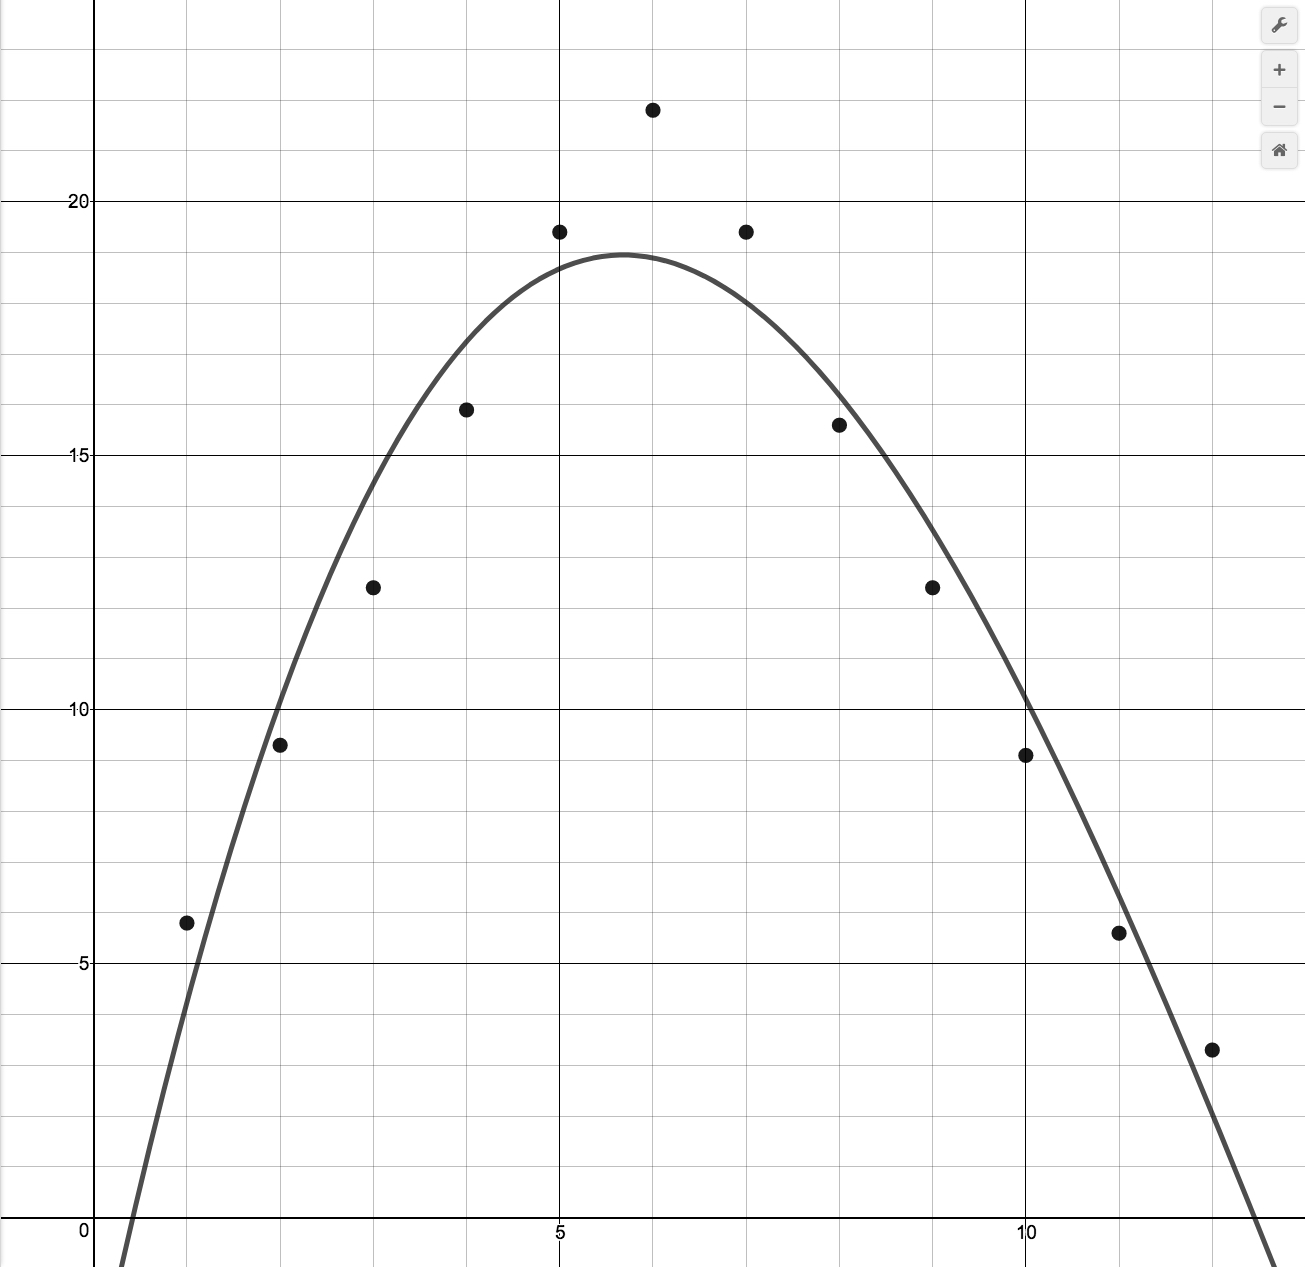
\includegraphics[width=2.5in]{./GraphsofPolynomialsGraphics/DaylightRegCubic.jpg} \hspace{.25in} & 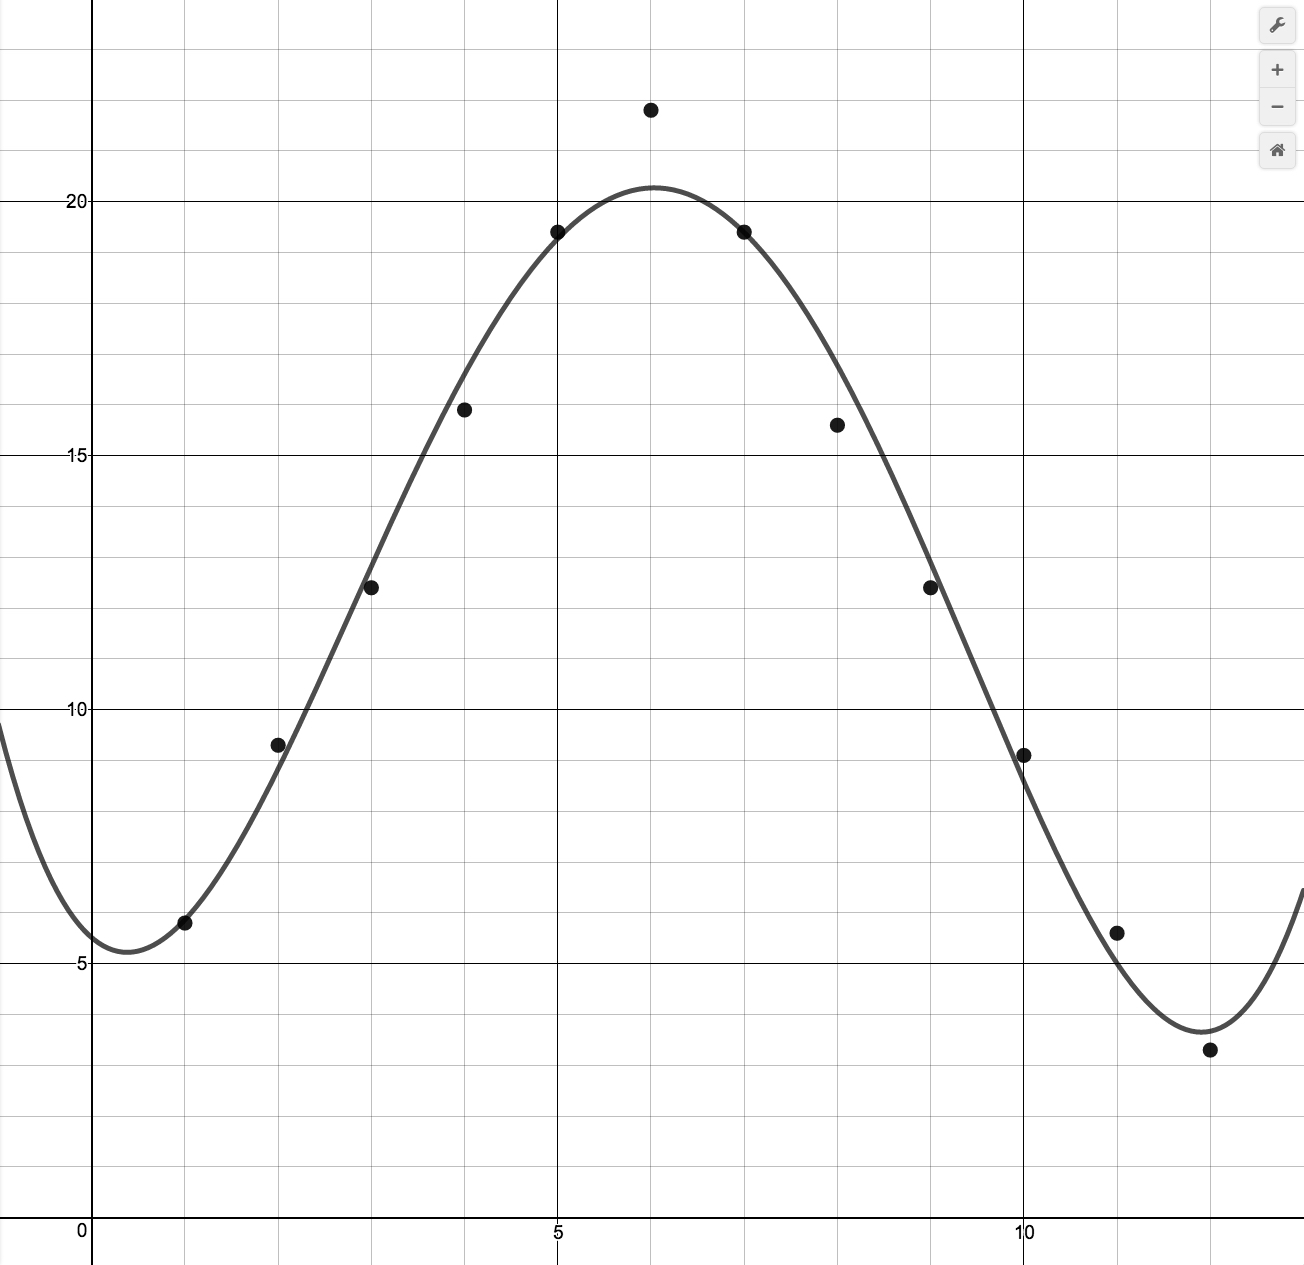
\includegraphics[width=2.5in]{./GraphsofPolynomialsGraphics/DaylightRegQuartic.jpg} \\

$y = p_{\mbox{\tiny $3$}}(x)$ \hspace{.25in} & $y = p_{\mbox{\tiny $4$}}(x)$ \\

\end{tabular}

\end{center}

\newpage

\item \begin{enumerate}

\item The scatter plot is shown below with each of the three regression models.

\item The quadratic model is $P_{\mbox{\tiny $2$}}(x) = -0.021x^{2} + 0.241x + 0.956$, $R^{2} = 0.7771$. \\
The cubic model is $P_{\mbox{\tiny $3$}}(x) = 0.005x^{3} - 0.103x^{2} + 0.602x + 0.573$,  $R^{2} = 0.9815$. \\
The quartic model is $P_{\mbox{\tiny $4$}}(x) = -0.000969x^{4} + 0.0253x^{3} - 0.240x^{2} + 0.944x + 0.330$,  $R^{2} = 0.9993$.

\item The models give maximums: $P_{\mbox{\tiny $2$}}(5.737) \approx 1.648$, $P_{\mbox{\tiny $3$}}(4.232) \approx 1.657$ and $P_{\mbox{\tiny $4$}}(3.784) \approx 1.630$.
\end{enumerate}



\hspace{-.1in} \begin{tabular}{ccc}

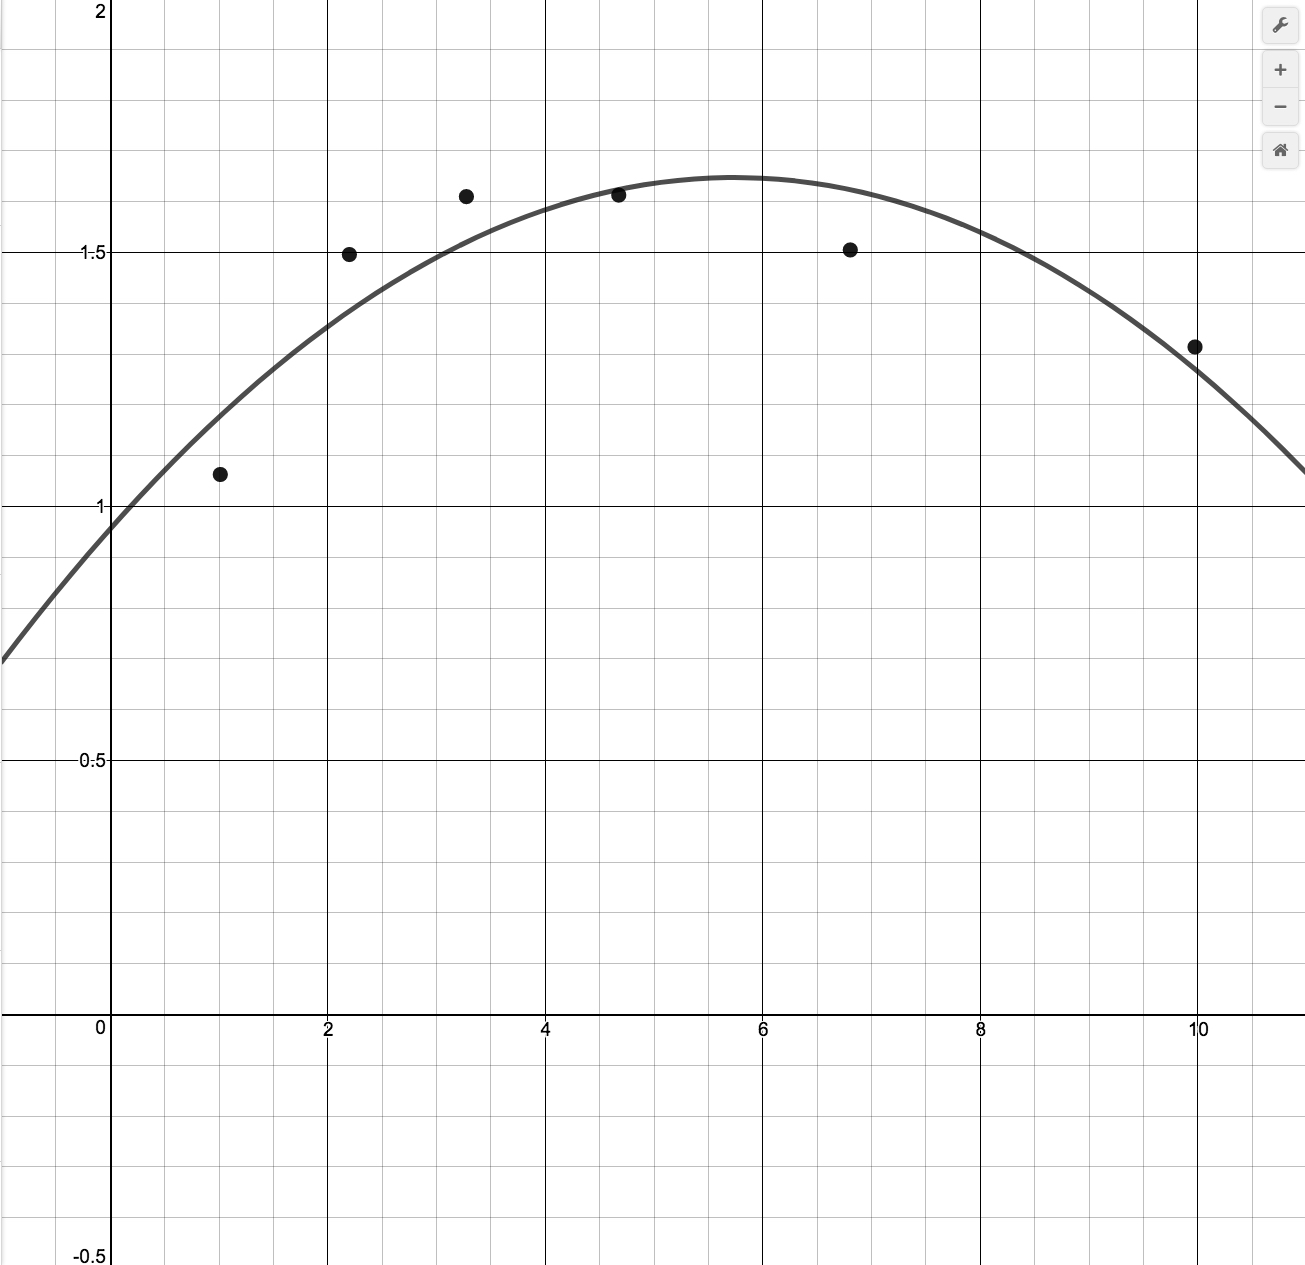
\includegraphics[width=1.8in]{./GraphsofPolynomialsGraphics/CircuitRegQuadratic.jpg} \hspace{.1in} &
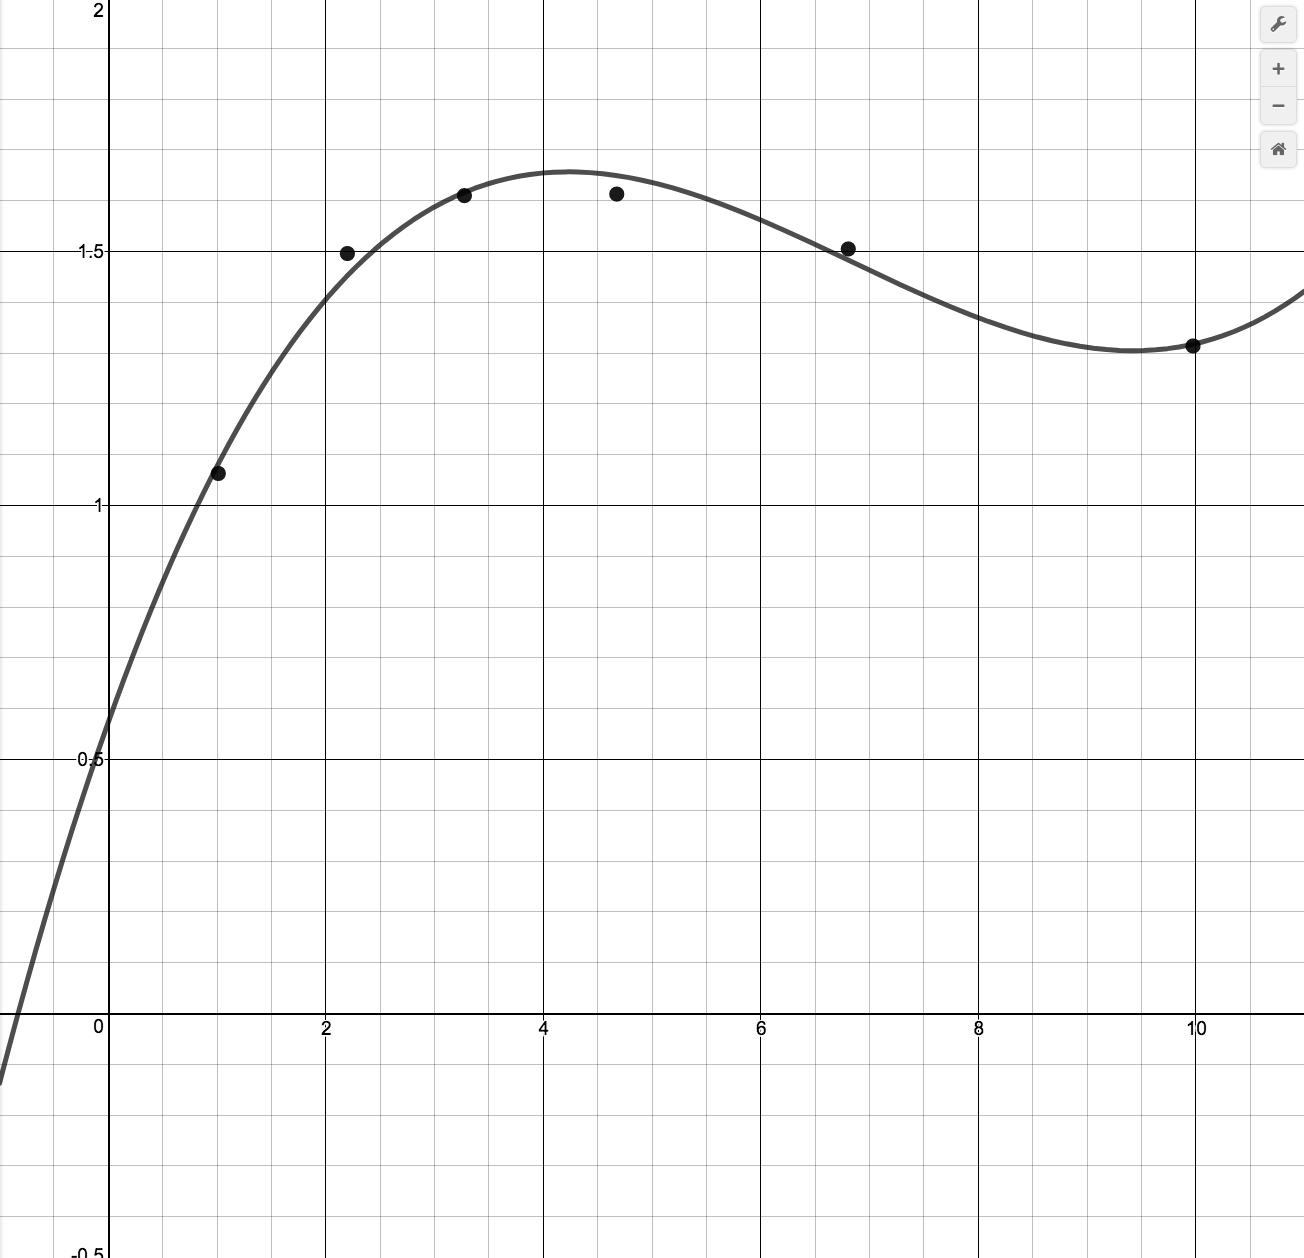
\includegraphics[width=1.8in]{./GraphsofPolynomialsGraphics/CircuitRegCubic.jpg} \hspace{.1in} &
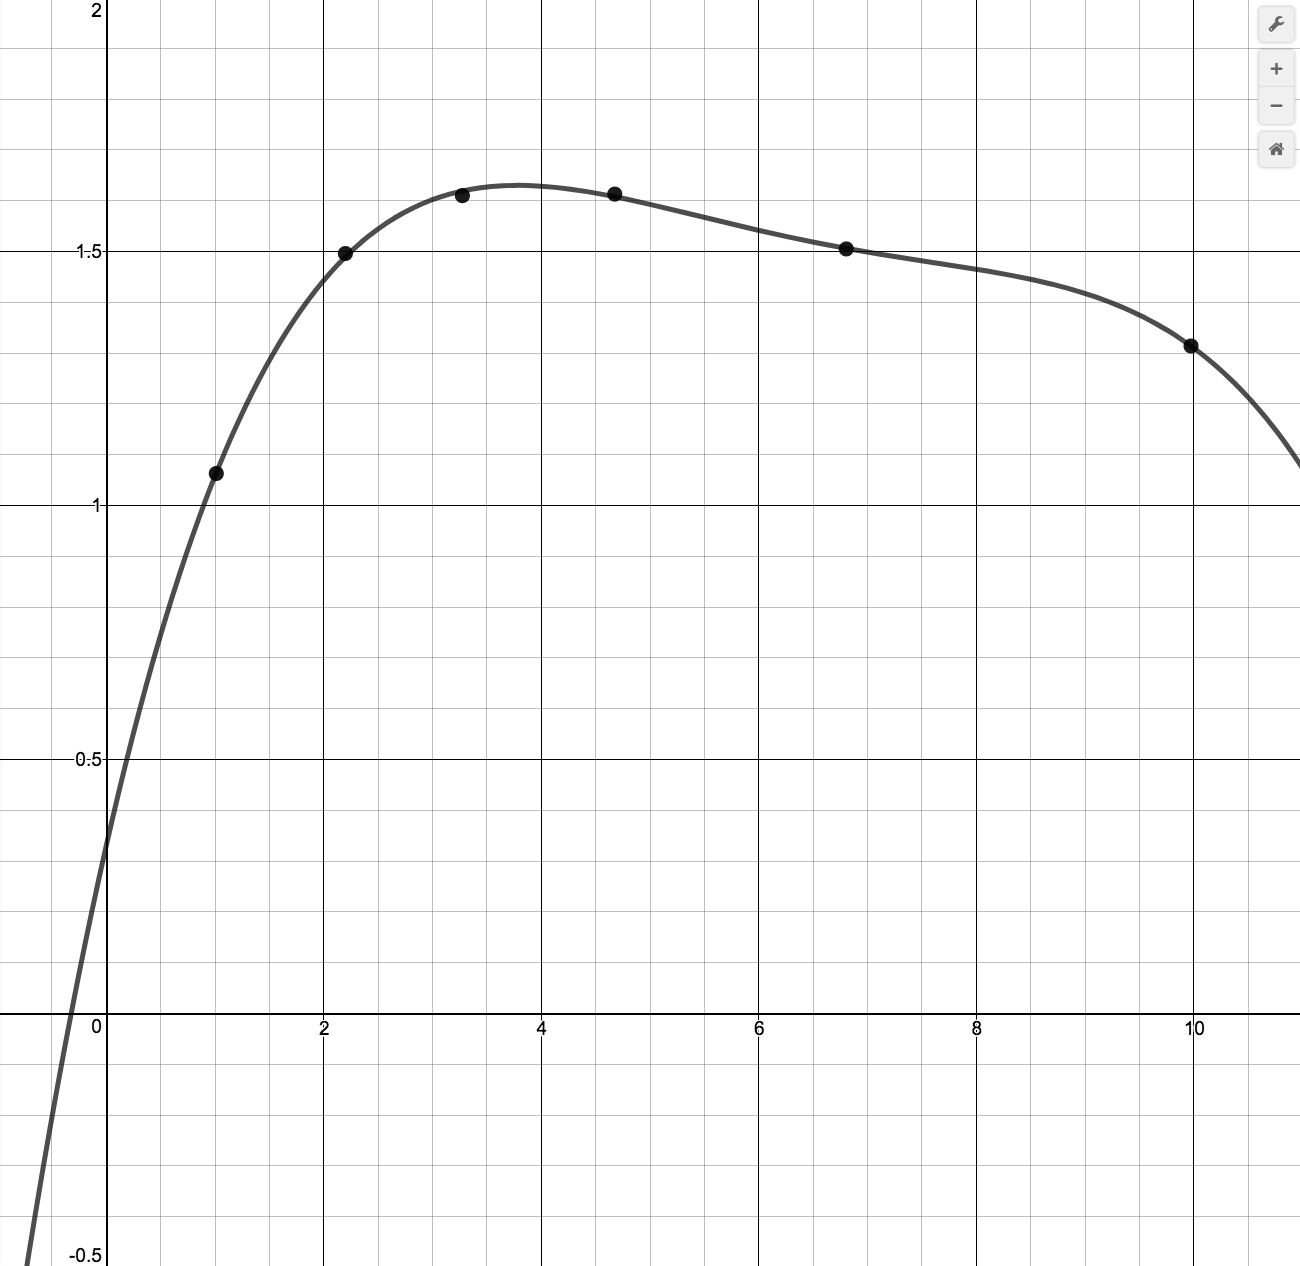
\includegraphics[width=1.8in]{./GraphsofPolynomialsGraphics/CircuitRegQuartic.jpg} \\

$y = P_{\mbox{\tiny $2$}}(x)$ \hspace{.1in} & $y = P_{\mbox{\tiny $3$}}(x)$ & $y = P_{\mbox{\tiny $4$}}(x)$\\

\end{tabular}

\item \begin{enumerate}

\item   $\ds{\lim_{x \rightarrow - \infty} p(x)  = -\infty}$  and $\ds{\lim_{x \rightarrow  \infty} p(x)  = -\infty}$

\item The zeros appear to be: $x=-1.5$, even multiplicity - probably $2$ since it doesn't `look like' the graph is very flat near $x = 2$;  $x=0$, odd multiplicity - probably $1$ since the graph seems fairly linear as it passes through the origin;  $x=1$ odd multiplicity - probably $3$ or higher since the graph seems fairly `flat' near $x = 1$.

\item  local minimum:  approximately $(-0.773, -2.888)$;  local maximums:  approximately $(-1.5,0)$, and $(0.32, 0.532)$

\item  Based on the graph, even degree (at least $6$ based on multiplicities) with a negative leading coefficient based on the end behavior.

\item  We only have a \textit{portion} of the graph represented here.

\end{enumerate}

\addtocounter{enumi}{1}

\item We are looking for the largest open interval containing $x = -0.235$ for which the graph of $y = p(x)$ is at or above $y=-1.121$.  Since each of the gridlines on the $x$-axis correspond to $0.2$ units, we approximate this interval as  $(-1.25 \, \text{ish}, 1.1 \, \text{ish})$.

\addtocounter{enumi}{4}

\item 

\begin{multicols}{2}
\begin{enumerate} \addtocounter{enumii}{2} 
\item $L(x) = x^2$


\item $L(x) = x+1$

\end{enumerate}
\end{multicols}

\end{enumerate}
